\begin{figure*}[!hbt]
  \centering
  \subfigure[Runtime on consecutive batch updates of size $10^{-5}|E_T|$]{
    \label{fig:temporal-sx-mathoverflow--runtime5}
    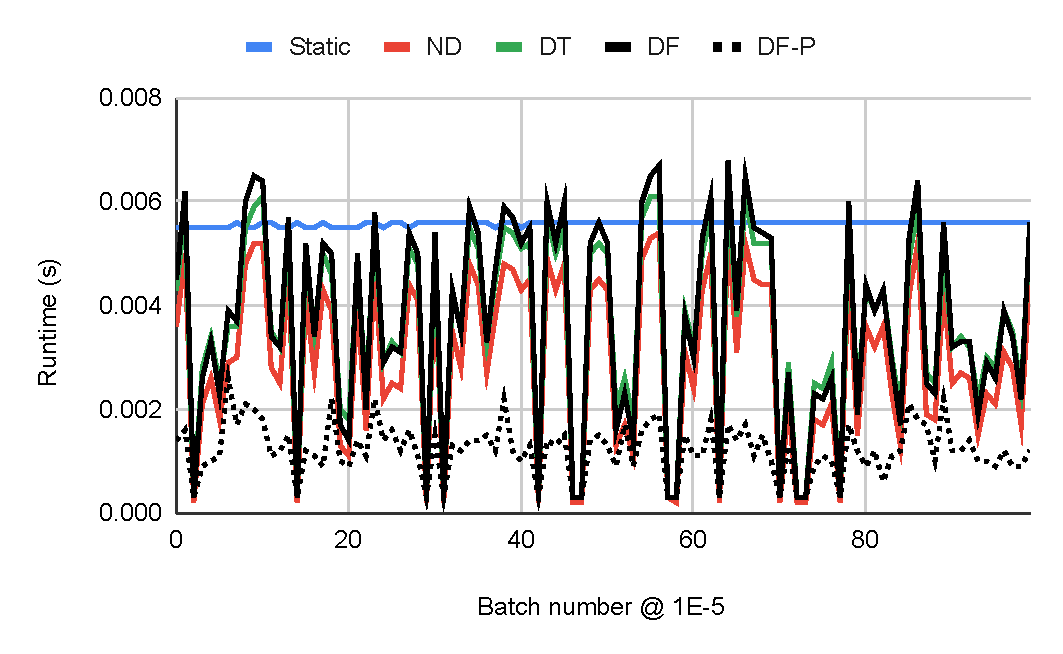
\includegraphics[width=0.48\linewidth]{out/temporal-sx-mathoverflow-runtime5.pdf}
  }
  \subfigure[Error in ranks obtained on consecutive batch updates of size $10^{-5}|E_T|$]{
    \label{fig:temporal-sx-mathoverflow--error5}
    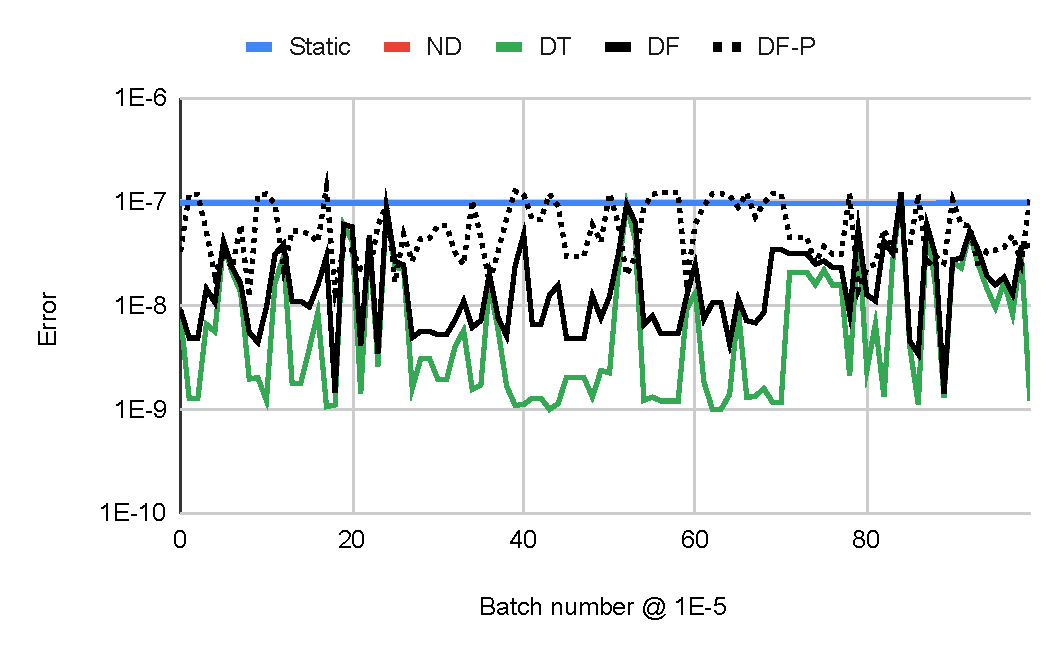
\includegraphics[width=0.48\linewidth]{out/temporal-sx-mathoverflow-error5.pdf}
  } \\[2ex]
  \subfigure[Runtime on consecutive batch updates of size $10^{-4}|E_T|$]{
    \label{fig:temporal-sx-mathoverflow--runtime4}
    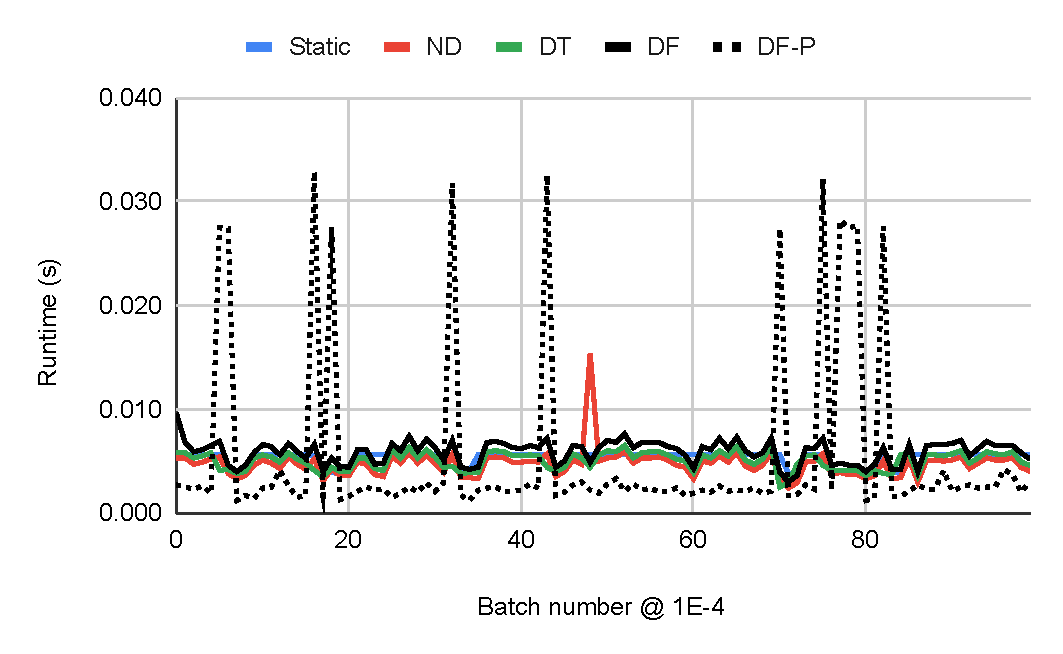
\includegraphics[width=0.48\linewidth]{out/temporal-sx-mathoverflow-runtime4.pdf}
  }
  \subfigure[Error in ranks obtained on consecutive batch updates of size $10^{-4}|E_T|$]{
    \label{fig:temporal-sx-mathoverflow--error4}
    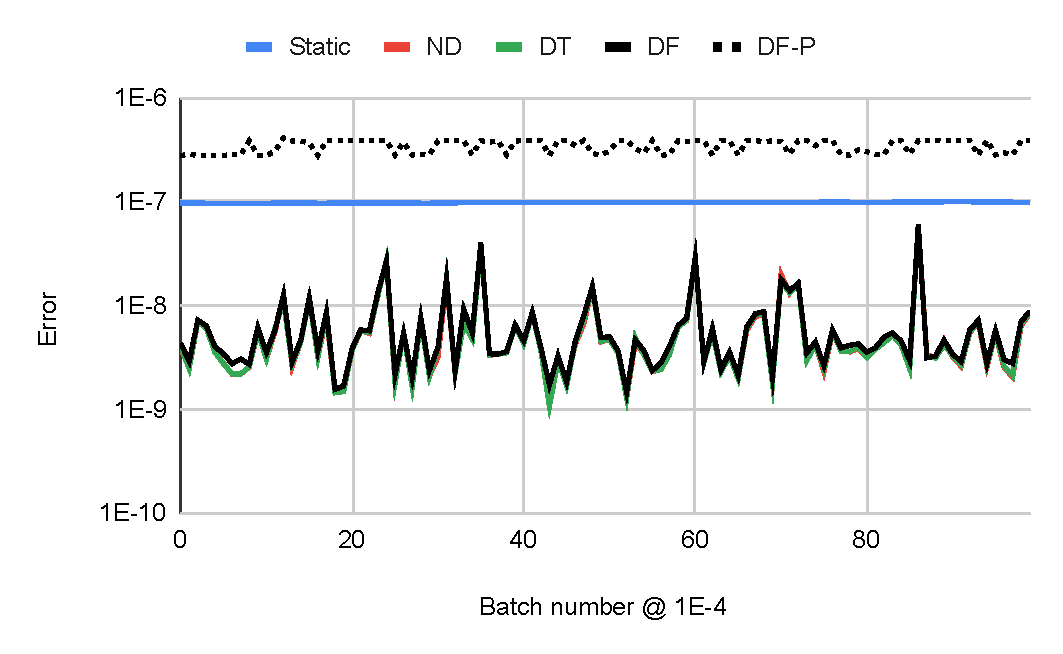
\includegraphics[width=0.48\linewidth]{out/temporal-sx-mathoverflow-error4.pdf}
  } \\[2ex]
  \subfigure[Runtime on consecutive batch updates of size $10^{-3}|E_T|$]{
    \label{fig:temporal-sx-mathoverflow--runtime3}
    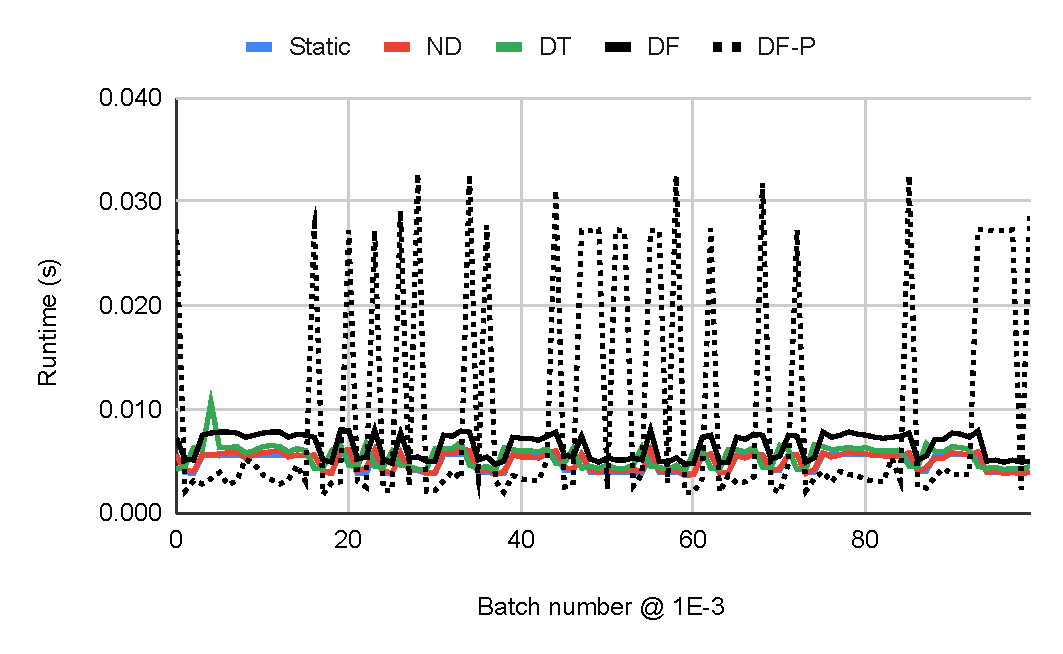
\includegraphics[width=0.48\linewidth]{out/temporal-sx-mathoverflow-runtime3.pdf}
  }
  \subfigure[Error in ranks obtained on consecutive batch updates of size $10^{-3}|E_T|$]{
    \label{fig:temporal-sx-mathoverflow--error3}
    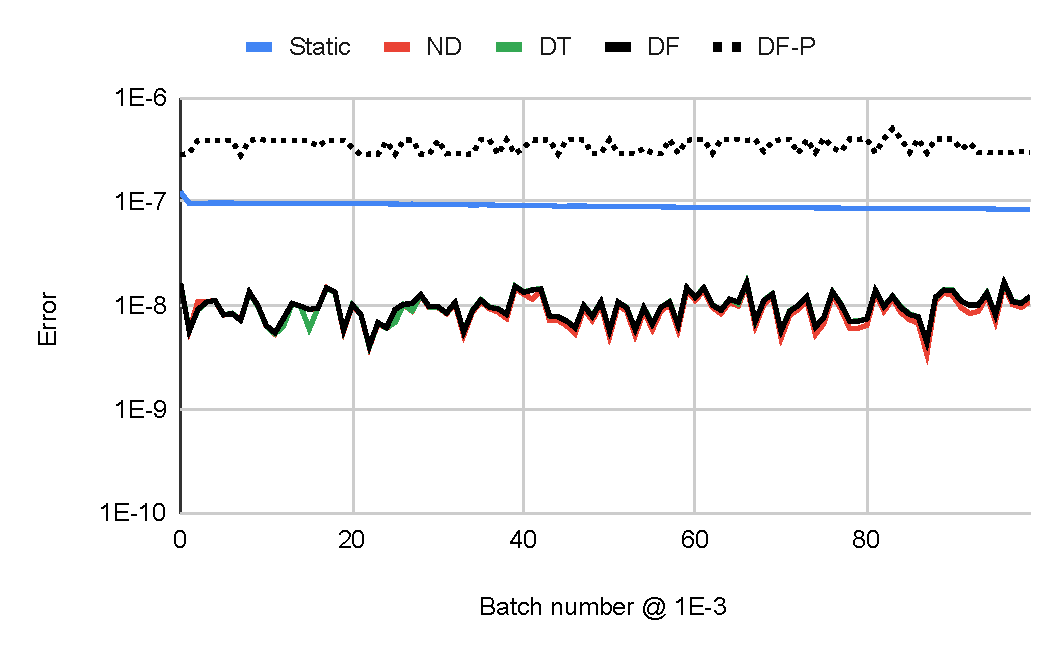
\includegraphics[width=0.48\linewidth]{out/temporal-sx-mathoverflow-error3.pdf}
  } \\[-2ex]
  \caption{Runtime and Error in ranks obtained with \textit{Static}, \textit{Naive-dynamic (ND)}, \textit{Dynamic Traversal (DT)}, our improved \textit{Dynamic Frontier (DF)}, and our improved \textit{Dynamic Frontier with Pruning (DF-P)} PageRank on the \textit{sx-mathoverflow} dynamic graph. The size of batch updates range from $10^{-5}|E_T|$ to $10^{-3}|E_T|$. The rank error with each approach is measured relative to ranks obtained with a reference Static PageRank run, as detailed in Section \ref{sec:measurement}.}
  \label{fig:temporal-sx-mathoverflow}
\end{figure*}
